% !TEX root = recipeUnderstanding.tex

\section{Introduction}
Human communication takes many forms, including language and vision. For instance, explaining ``how-to'' perform a certain task can be communicated via language (e.g., Do-It-Yourself books) as well as visual (e.g., instructional YouTube videos) information. Regardless of the form, such human-generated communication is generally structured and has a clear beginning, end, and a set of steps in between. Parsing such communication into its semantic steps is the key to understand human activities. 

%With a large amount of instructional video collections, we present a method to ground and parse them into semantically meaningful actions.


%In this paper, we propose a method for decomposing a video into semantically meaningful steps in a fully unsupervised manner.

% both used.
%  With large amount of document collections, there is a huge body of work dedicated to understanding language \cite{xx,nap}.
%
% Language and vision are the two main modalities employed for this structured communication by
%% AMIR: paragraph Could be removed
Language and vision often provide different, but correlating and complementary information. Challenge lies in that both video frames and language (from subtitles\footnote{generated either via Automatic Speech Recognition (ASR) or by the user, are now available for most YouTube videos.}) are only a noisy, partial observation of the actions being performed. However, the complementary nature of language and vision gives the opportunity to robustly understand the activities only from these partial observations. In this paper, we present a unified model, considering both of the modalities, in order to parse human activities into activity steps with no form of supervision.

%

%requires us to model them jointly. We present a unified model, learnt in a fully unsupervised manner, in order to jointly use these two modalities.

% Furthermore they are
% We utilize these two modalities (video frames and imperfect automatically generated subtitles) in a unified manner in our framework;
% We qualitatively and quantitatively argue that a joint inference is crucial for a successful semantic parsing, particularly when no supervision is employed.


%  the proposed approach on instructional videos from YouTube (\eg, ``Making panckage'', ``How to tie a bow tie'') as they typically have clear steps and provide concrete grounds for demonstrating a semantically meaningful parsing. These videos are often long and manifest a high intra-class variability yet the underlying steps remains well-defined and structured, similar to almost all human communications.

\begin{figure}[h!]
  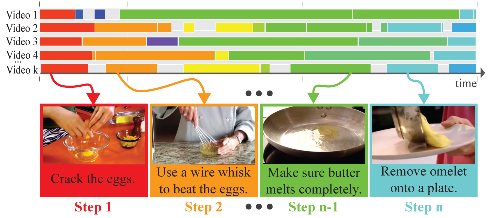
\includegraphics[width=0.48\textwidth]{Figure_1_flattened}
  \caption{Given a large video collection, we discover semantic activity steps without any supervision by using available multi-modal information (visual frames and subtitles). We also parse each video based on the discovered steps.}
  \label{teaser}
\end{figure}


The key idea in our approach is the observation that the largecollection of videos, pertaining to the same activity class, typically include only a few objective activity steps, and the variability is the result of exponentially many ways of generating videos from activity steps through subset selection and time ordering. We study this construction based on the large-scale information available in YouTube in the form of instructional videos  (\eg, ``Making panckage'', ``How to tie a bow tie''). Instructional videos have many desirable properties like the volume of the information (e.g., YouTube has 281.000 videos for \emph{"How to tie a bow tie"}) and a well defined notion of activity step.  However, the proposed parsing method is applicable to any type of videos as long as they are composed of a set of steps.

%I think the story line idea is not that strong anymore, we are discovering and parsing
The output of our method can be seen as the semantic ``storyline'' of a rather long and complex video collection (see Fig. \ref{fig:teaser}). This storyline provides what particular steps are taking place in the video collections, when they are occurring, and what their semantic meaning is (\emph{what-when-how}). This method also puts multiple videos performing the same overall task in common ground (i.e., the semantic steps’ space) and capture their high-level similarity.

%, and therefore, provide a \emph{categorical} storyline as well.

In the proposed approach, given a collection of videos, we first generate a set of language and visual atoms. These atoms are the result of relating object proposals from each frame as well as detecting the frequent words from subtitles. We then employ a generative \emph{beta process mixture model}, which identifies the activity steps shared among the videos of the same category based on a representation using learned atoms. In our method, we do neither use any spatial or temporal label on actions/steps nor any labels on object categories. We later learn a Markov language model to provide a textual description of the activity steps based on the language atoms it frequently uses.

%Still semantic storyline is not the story anymore
%provide a semantic storyline for a complex video collection. 
This work is the first to discover activity steps for a complex video collection with no supervision over activions and/or objects. We are also the first to approach this problem in a multimodal (joint language and vision) manner. In addition, our method is capable of providing a caption describing the steps; our approach to captioning is fundamentally different from the majority of existing video/image-to-text work in two aspects: 1) the captions are generated without any supervised caption-clip pairs, 2) our captions are \emph{descriptions} of the semantic steps, yet they are inferred from \emph{narrations}. This is different from the existing captioning work as their reference data is also descriptive of the visual information, while the narration over videos often provides complementary information to the visuals and is not necessarily descriptive.

%Leaning the instructions of a novel non-trivial task is both a challenge and a necessity for both humans and autonomous systems. This necessity resulted in many community generated instruction collections \cite{wikiHow,eHow} and expert curated recipe books\cite{recipeBook1,recipeBook2}. However, this instructions are generally based on a language modality and explains a single way of performing the task although there are variety of ways. On the other hand, online video storage services are full of unstructured instructional videos\footnote{YouTube has 281.000 videos for \emph{"How to tie a bow tie"}} covering variety of ways, environment conditions and view angles. Although there have been many successful attempts in detecting activities from videos \cite{act1,act2}, structural representation of such a large and useful video collection is not possible. In this paper, we focus on joint semantic representation of YouTube videos as a response to a single query. We specifically study the unsupervised joint-detection of the activities from a collection of YouTube videos.

%Understanding of the instructional videos, requires the careful processing of two complementary modalities namely language and the vision.  Luckily the target domain, YouTube videos, has unstructured subtitles as well. They are either generated by the content developer (5\% of the time) or automatically generated by using the Automatic Speech Recognition (ASR) software. The main limitations of the existing activity detection literature for this problem is scalability and representation level. Existing approaches are mainly supervised and requires extensive training set which is not tractable in the scale of YouTube videos. Moreover, current activity detection research focuses on the low-level visual features. However, such videos in the wild have objects with completely different texture and shape characteristics from wide range of views. Instead, we focus on extracting high-level visual semantic representations and using salient words occurring among the videos.

%We rely on the assumption that the videos collected as the response of a same instructional query, share similar activities performed by the similar objects. We start with the independent processing of the videos in order to create a large collection of visual object proposals and words. After the proposal generation, we jointly process the proposal collections and words to detect the visual objects and words which can be used to represent the unstructured information. Since we rely on high-level information instead of the low-level features, the resulting objects represent the semantic information instead of visual characteristic. By using the extracted objects, we compute the holistic representation of the multi-modal information in each frame.

%Moving from frame-wise visual understanding to activity understanding, requires the joint processing of all the videos with the temporal information. In order to exploit the temporal information, we model each video as a Hidden Markov Model using state space of activities. Since we assume that the videos share some of the activities and we have no supervision, we use a model based on \emph{beta process mixture model}. Our model jointly learn the activities and detect them in the videos. Moreover, it does not require prior knowledge over the number of activities.
